%======================================================%
%   Beamer Presentation
%   LaTeX Template
%   compile using PDFTeXify, PDFLaTeX or XeLaTeX
%======================================================%

%--------------------------------------------------------------------------------
%   PACKAGES AND THEMES
%--------------------------------------------------------------------------------

\documentclass[noamsthm,notheorems,11pt,compress,fontset=windows]{beamer}


%------- Beamer theme ------
%\usetheme{Frankfurt}
%\usetheme{Montpellier}
%\usetheme{Warsaw}
%\usetheme{CambridgeUS}
%\usetheme{Boadilla}

%------- Color theme ------
%\usecolortheme{rose}
%\usecolortheme{orchid}
%\usecolortheme{lily}
%\usecolortheme{whale}
%\usecolortheme{dolphin}
%\usecolortheme{seahorse}

%\usetheme{boxes}
%\setbeamercovered{transparent}
%\usefonttheme[onlymath]{serif}
\usefonttheme{serif}
\usefonttheme{professionalfonts}

\setbeamersize{text margin left=0.5cm, text margin right=0.5cm}

%\setbeamertemplate{headline}{}
%\setbeamertemplate{footline}{}
\setbeamertemplate{blocks}[rounded][shadow=true]
\setbeamertemplate{navigation symbols}{}
\setbeamertemplate{itemize items}[circle]  % ball, circle
\setbeamertemplate{enumerate items}[default]
%\setbeamertemplate{section in toc}[square]

%---------- 定义目录 ----------
\setbeamertemplate{section in toc}{
  \leavevmode\leftskip=2.5em%
  \llap{%
    \usebeamerfont*{section number projected}%
    \usebeamercolor{section number projected}%
    \begin{pgfpicture}{-1ex}{-0.2ex}{1ex}{2ex}
      %\color{structure.fg}
      \pgfpathcircle{\pgfpoint{0pt}{.75ex}}{1.3ex}
      \pgfusepath{fill}
      \pgftext[base]{\color{white}\inserttocsectionnumber}
    \end{pgfpicture}\kern2ex%
  }%
  \inserttocsection\par
}

%---------- 定义颜色 ----------
\definecolor{deepblue}{rgb}{0,0.3,0.58}
\definecolor{darkblue}{rgb}{0.02,0.24,0.44}
\definecolor{footer}{rgb}{0.5,0.2,0.5}
\definecolor{bgblue1}{rgb}{0,0.23,0.44}
\definecolor{bgblue2}{rgb}{0,0.15,0.29}
%\definecolor{darkorange}{rgb}{0.80,0.4,0.1}
\definecolor{darkred}{rgb}{0.90,0.1,0.1}
\definecolor{darkgreen}{rgb}{0.02,0.18,0.20}
\setbeamercolor{structure}{fg=deepblue}
\setbeamercolor{alerted text}{fg=darkred}

\setbeamercolor{title}{fg=deepblue,bg=gray!12}
\setbeamercolor{subtitle}{fg=deepblue!80,bg=gray!12}
%\setbeamercolor{institute}{fg=white}
%\setbeamercolor{author}{fg=white}
%\setbeamercolor{date}{fg=white}
\setbeamercolor{frametitle}{fg=deepblue,bg=gray!12}
%\setbeamercolor{section in head/foot}{bg=bgblue2,fg=white}
\setbeamercolor{section in head/foot}{bg=bgblue2!50!bgblue1,fg=white}
\setbeamertemplate{section in head/foot shaded}{\color{gray}
\usebeamertemplate{section in head/foot}}

\setbeamercolor{title in head/foot}{bg=bgblue2,fg=black!5}
\setbeamercolor{author in head/foot}{bg=bgblue1,fg=black!5}
\setbeamercolor{date in head/foot}{bg=bgblue1,fg=black!5}
\setbeamercolor{section in toc}{fg=structure.fg}

%\setbeamertemplate{section in toc}[sections numbered]
%\setbeamertemplate{subsection in toc}[subsections numbered]
%\setbeamertemplate{section in toc}[ball unnumbered]
%\setbeamertemplate{subsection in toc}[ball unnumbered]

% change the style of headline
\setbeamertemplate{headline}{
  \begin{beamercolorbox}[ht=4.5ex]{section in head/foot}
  \vskip3pt\insertsectionnavigationhorizontal{\textwidth}{}{}\vskip2pt
  %\vskip2pt\insertnavigation{\paperwidth}\vskip2pt
  \end{beamercolorbox}
}

% change the style of frametitle
\makeatletter
\setbeamertemplate{frametitle}{%
  \ifbeamercolorempty[bg]{frametitle}{}{\nointerlineskip}%
  \@tempdima=\textwidth%
  \advance\@tempdima by\beamer@leftmargin%
  \advance\@tempdima by\beamer@rightmargin%
  \hfill%
  \begin{beamercolorbox}[wd=\paperwidth,sep=8pt,left]{frametitle}
    \usebeamerfont{frametitle}%
    \vbox{}\vskip-1.2ex%
    \if@tempswa\else\csname beamer@fteleft\endcsname\fi%
    \strut\insertframetitle\strut\par%
    {%
      \ifx\insertframesubtitle\@empty%
      \else%
      {\usebeamerfont{framesubtitle}\usebeamercolor[fg]{framesubtitle}\strut\insertframesubtitle\strut\par}%
      \fi
    }%
    \vskip-1ex%
    \if@tempswa\else\vskip-8pt\fi
  \end{beamercolorbox}%
}
\makeatother

% change the style of footline
\makeatletter
\setbeamertemplate{footline}{%
  \leavevmode%
  \begin{beamercolorbox}[wd=0.3\paperwidth,ht=2.25ex,dp=1ex,center]{author in head/foot}%
    \usebeamerfont{title in head/foot} ~~\insertshortauthor\ifx\insertshortinstitute\empty\else\expandafter
    \ifblank\expandafter{\beamer@shortinstitute}{}{~(\insertshortinstitute)}\fi
    \hfill
  \end{beamercolorbox}%
  \begin{beamercolorbox}[wd=0.4\paperwidth,ht=2.25ex,dp=1ex,center]{title in head/foot}%
    \usebeamerfont{title in head/foot}\centering \insertshorttitle
  \end{beamercolorbox}%
  \begin{beamercolorbox}[wd=0.3\paperwidth,ht=2.25ex,dp=1ex,right]{date in head/foot}%
    \usebeamerfont{date in head/foot}\hfill\insertshortdate{}\hfill %\kern1ex
    \makebox[3em][r]{\insertframenumber\,/\,\inserttotalframenumber}\kern2ex
  \end{beamercolorbox}%
  \vskip0pt%
}
\makeatother


%--------- 宏包  ----------
\usepackage[UTF8]{ctex}
%\usepackage[english]{babel}
\usepackage{amsmath,amssymb,version}
\usepackage{graphicx,fancybox,mathrsfs,multirow}
\usepackage{booktabs}
\usepackage{epsfig,epstopdf}
\usepackage{url,hyperref}
\usepackage{tabularx,array,makecell}
\usepackage{color,xcolor}
\usepackage{cases}
\usepackage{caption}
\usepackage{mathtools}
\usepackage{tikz}

%---------- 定义行距 ----------
%\renewcommand{\baselinestretch}{1.15}

%---------- 定义表格新命令 ----------
\newcolumntype{P}[1]{>{\centering \arraybackslash}p{#1}}
\newcolumntype{L}{X}
\newcolumntype{C}{>{\centering \arraybackslash}X}
\newcolumntype{R}{>{\raggedleft \arraybackslash}X}

%---------- Caption Setting ----------
\captionsetup[figure]{position=bottom,skip={6pt}}
\captionsetup[table]{position=top,skip={3pt}}

%---------- 设置字体  ----------
\setbeamerfont{normal text}{family=\rmfamily}
\setbeamerfont{frametitle}{family=\rmfamily,series=\bfseries}
\setbeamerfont{title}{family=\rmfamily,series=\bfseries}
\setbeamerfont{subtitle}{family=\rmfamily,series=\bfseries}
\setbeamerfont{institute}{family=\rmfamily}
\setbeamerfont{author}{family=\rmfamily}
\setbeamerfont{date}{family=\rmfamily}
\setbeamerfont{headline}{family=\sffamily\heiti}
\setbeamerfont{footline}{family=\rmfamily} %\kaishu
\setbeamerfont{section in toc}{family=\rmfamily,series=\bfseries}
\setbeamerfont{subsection in toc}{family=\rmfamily}
\AtBeginDocument{\usebeamerfont{normal text}}

\setbeamertemplate{caption}[numbered]
\numberwithin{figure}{section}
\numberwithin{table}{section}
\numberwithin{equation}{section}

\graphicspath{{./figures/}}

%----- fix label spacing -----
\makeatletter
\def\beamer@inserttarget#1{%
  \ifbeamer@inframe%
    #1%
  \else% defer to next frame
    \expandafter\gdef\expandafter\beamer@framehypertargets
    \expandafter{\beamer@framehypertargets#1}%
  \fi%
}
\makeatother

%----- 定义定理颜色 -----
\definecolor{bgcolor1}{rgb}{0.95,0.95,1}
\definecolor{lncolor1}{rgb}{0.63,0.58,0}
\definecolor{bgcolor2}{rgb}{0.95,0.95,0.95}
\definecolor{lncolor2}{rgb}{0.95,0.4,0.1}
\definecolor{bgcolor3}{rgb}{0.9,1,0.9}
\definecolor{lncolor3}{rgb}{0.3,0.3,0.3}

%---------- 定理设置  --------------
\usepackage[framemethod=tikz]{mdframed}
\usepackage[amsmath,thref,thmmarks,hyperref]{ntheorem}
\theorempreskipamount1.2em  % spacing before the environment
\theorempostskipamount0em  % spacing after the environment
\theorempostwork{\noindent}
\theoremstyle{plain} %break,plain,nonumberbreak
\if@docn
\theoremheaderfont{\color{structure.fg}\bfseries} %\upshape
\else
\theoremheaderfont{\color{structure.fg}\bfseries} %\upshape
\fi
\theorembodyfont{} %\itshape %\setlength{\baselineskip}{15pt}
\theoremindent0em
\theoremseparator{.} %if break -> add \vspace{0.2em}
\theoremnumbering{arabic}
\colorlet{thmcolor}{darkgreen}
\newmdtheoremenv[linecolor=lncolor1,middlelinewidth=0.5pt,
    roundcorner=1pt,backgroundcolor=bgcolor1,%
    innertopmargin=0.4em,innerbottommargin=0.4em,%
    innerleftmargin=5pt,innerrightmargin=5pt,%
    skipbelow=0.5em,skipabove=1em,%
    splittopskip=\topskip,ntheorem]{theorem}%
    {定理}%[section]
\newmdtheoremenv[linecolor=lncolor1,middlelinewidth=0.5pt,
    roundcorner=1pt,backgroundcolor=bgcolor1,%
    innertopmargin=0.4em,innerbottommargin=0.4em,%
    innerleftmargin=5pt,innerrightmargin=5pt,%
    skipbelow=0.5em,skipabove=1em,%
    splittopskip=\topskip,ntheorem]{corollary}%
    {推论}%[section]
\newmdtheoremenv[linecolor=lncolor1,middlelinewidth=0.5pt,
    roundcorner=1pt,backgroundcolor=bgcolor1,%
    innertopmargin=0.4em,innerbottommargin=0.4em,%
    innerleftmargin=5pt,innerrightmargin=5pt,%
    skipbelow=0.5em,skipabove=1em,%
    splittopskip=\topskip,ntheorem]{lemma}%
    {引理}%[section]
\newmdtheoremenv[linecolor=lncolor2,middlelinewidth=0.5pt,
    roundcorner=1pt,backgroundcolor=bgcolor2,%
    innertopmargin=0.4em,innerbottommargin=0.4em,%
    innerleftmargin=5pt,innerrightmargin=5pt,%
    skipbelow=0.5em,skipabove=1em,%
    splittopskip=\topskip,ntheorem]{proposition}%
    {命题}%[section]
\newmdtheoremenv[linecolor=lncolor3,middlelinewidth=0.5pt,
    roundcorner=1pt,backgroundcolor=bgcolor3,%
    innertopmargin=0.4em,innerbottommargin=0.4em,%
    innerleftmargin=5pt,innerrightmargin=5pt,%
    skipbelow=0.5em,skipabove=1em,%
    splittopskip=\topskip,ntheorem]{definition}%
    {定义}%[section]
\newmdtheoremenv[linecolor=white,middlelinewidth=0.5pt,
    roundcorner=2pt,backgroundcolor=none,%
    innertopmargin=0em,innerbottommargin=0em,%
    innerleftmargin=0pt,innerrightmargin=0pt,%
    skipbelow=0.5em,skipabove=1em,%
    splittopskip=\topskip,ntheorem]{example}%
    {例}%[section]

%---------- 证明和解环境 ----------
\newenvironment{proof}[1][证明]{\par\textbf{#1:}%
\enspace\ignorespaces}{\par}
\newenvironment{solution}{\par\textbf{解:}%
\enspace\ignorespaces}{\par}

%---------- 证明符号 ----------
\newcommand{\QED}{\hfill\ensuremath{\square}}

%---------- 调节公式的间距 ----------
\AtBeginDocument{
	\setlength{\abovedisplayskip}{6pt plus 1pt minus 1pt}
	\setlength{\belowdisplayskip}{6pt plus 1pt minus 1pt}
	\setlength{\abovedisplayshortskip}{2pt}
	\setlength{\belowdisplayshortskip}{2pt}
	\setlength{\arraycolsep}{2pt}
}


\makeatletter
\newcommand\HUGE{\@setfontsize\Huge{28}{32}}
\makeatother


%\AtBeginSection[]{
%\begin{frame}
%  \frametitle{目录}
%  \tableofcontents[currentsection,currentsubsection,subsectionstyle=show/show/shaded]
%  \addtocounter{framenumber}{-1}
%\end{frame}
%}


%---------- 自定义命令 ----------
\newcommand{\red}[1]{\textcolor{red}{#1}}
\newcommand{\blue}[1]{\textcolor{blue}{#1}}


%--------------------------------------------------------------------------------
%	TITLE PAGE
%--------------------------------------------------------------------------------

\title[Redes Sem Fio]{Eficiência, Justiça e Exclusão em Escalonadores 5G sob Cargas Variaveis}

\author[UFCA]
{    
    \vskip 4mm
    Ciência da Computação \vskip 1mm
    Redes Sem Fio \vskip 1mm
    Alex Reis, David Hudson, Luana Teles, Thiago Nerton, Victor Cleyton, Vitória Pontes
}
%\author[姓名]{报告人姓名}

%\institute[UFCA]{UFCA}
%\institute[学校名称]{\normalsize 学校名称}

\date[2026.8.20]{2026.8.20}


\begin{document}

% only change the spacing of body text
\setlength{\baselineskip}{15pt}


{%\setbeamertemplate{headline}{}
\begin{frame}
\titlepage % Print the title page as the first slide
\end{frame}}


\begin{frame}
\frametitle{Sumário}
\tableofcontents
\end{frame}


%--------------------------------------------------------------------------------
%	PRESENTATION SLIDES
%--------------------------------------------------------------------------------

%------------------------------------------------
\section{Introdução}
%------------------------------------------------
\begin{frame}{Problema}
Em \textbf{sistemas 5G}, o escalonador precisa decidir qual usuário recebe os recursos em cada intervalo de transmissão.

\vspace{3mm}

\begin{itemize}
    \item Existem três abordagens básicas:
    \begin{itemize}
        \item \textbf{Round Robin}: distribuição cíclica dos recursos, ignorando a qualidade do canal;
        \item \textbf{MaxCI}: prioriza quem tem a melhor condição instantânea do canal;
        \item \textbf{Proportional Fair}: compromisso entre oportunidade instantânea e histórico de serviço do usuário.
    \end{itemize}
    \end{itemize}

\end{frame}

%------------------------------------------------


\begin{frame}{Problema}

\begin{alertblock}{}
Essas estratégias podem gerar um conflito entre \textbf{eficiência} e \textbf{justiça}.
\end{alertblock}

\vspace{3mm}

Esse conflito pode mudar quando:
\begin{itemize}
    \item Aumenta a carga de \textbf{UEs};
    \item Os usuários possuem \textbf{condições médias de canal diferentes};
    \item A justiça é avaliada por \textbf{métricas diferentes}.
\end{itemize}

\vspace{0.3cm}

\begin{block}{Pergunta central}
Como carga, heterogeneidade espacial e definição de justiça
alteram a comparação entre RR, MaxCI e PF?
\end{block}

\end{frame}

%------------------------------------------------

\begin{frame}{Motivação}
    \begin{itemize} 
        \item Entender como \textbf{diferentes políticas de escalonamento} se comportam sob alta carga.
        
        \item A heterogeneidade do canal pode favorecer usuários com melhores condições, em detrimento de outros. Uma política que funciona bem em cenários homogêneos \textbf{pode falhar em cenários reais}.
        
        \item É importante analisar o \textbf{trade-off entre eficiência e justiça} entre diferentes políticas de escalonamento. 
        
    \end{itemize} 
    
    \begin{block}{Objetivo} Avaliar como carga e heterogeneidade do canal afetam esse trade-off em RR, MaxCI e PF. 
    \end{block} 
\end{frame}

%-----------------------------------------------

\section{Metodologia}
\begin{frame}{Condução do Experimento} 
    \textbf{Parâmetros Principais}
    \begin{itemize} 
        \item 5 cargas: 2, 4, 8, 16 e 32 usuários.
        \item 10.000 intervalos de transmissão (TTIs) por semente.
        \item 50 sementes aleatórias por condição.
        \item Canal Rayleigh em blocos gerados pelo Sionna.
        
    \end{itemize} 
    
    \begin{block}{Objetivo} Para cada semente aleatória, executamos RR, PF e MaxCI sobre a mesma realização de canal.
    \end{block} 
\end{frame}

%------------------------------------------------
\begin{frame}{Políticas e Métricas} 
    \textbf{Políticas}
    \begin{itemize} 
        \item \textbf{RR}: \( u_t = t \bmod N \), seleção cíclica, ignora o canal.
        \item \textbf{MaxCI}: \( u_t = \arg\max_u r_{u,t} \), seleciona a maior taxa instantânea.
        \item \textbf{PF}: \( u_t = \arg\max_u \frac{r_{u,t}}{T_u(t)} \), normaliza pela média histórica, com \beta = 0.98
    \vspace{2mm}
    \end{itemize} 
    \textbf{Métricas} \par
    Vazão agregada, JFI de slots, JFI de vazão, Índice de Gini, percentil 5 da vazão, UEs nunca atendidos, invervalos sem atendimento.
    
\end{frame}

%------------------------------------------------
\begin{frame}{Cenário Heterogêneo} 
    \textbf{Ganho relativo de potência dependente da distância:}
    \[
    g_u = \frac{(d_0 / \tilde{d}_u)^\alpha}{\frac{1}{N} \sum_v (d_0 / \tilde{d}_v)^\alpha}
    \]

    \begin{itemize} 
        \item \( d_u \) é a distância do usuário à estação base
        \item \( \alpha \) é o expoente de perda de percurso (variamos de 1,5 a 4,0)
        \item A normalização mantém o ganho médio unitário entre os usuários.
    \end{itemize} \par
    Criamos um \textbf{contraste controlado} entre usuários próximos e distantes.
    
\end{frame}

%------------------------------------------------

\section{Resultados}

\begin{frame}{Resultados - Cenário Homogêneo}

\begin{itemize}
    \item Com N=32, o \textbf{MaxCI} apresentou JFI de slots de 0,9972 e JFI de vazão de 0,9971. Nenhum dos 50 seeds produziu exclusão total de usuários.

    \item \textbf{MaxCI} tende a ser justa em horizontes longos; por simetria, todos têm a mesma chance de serem selecionados.

    \item Intervalo médio sem atendimento:

        \begin{itemize}
            \item RR: 32 TTIs
            \item PF: 63,8 TTIs
            \item MaxCI: 313,5 TTIs
        \end{itemize}

\end{itemize}

    \begin{block}{} Usuários do MaxCI podem ficar longos períodos sem serviço, mesmo que a média seja justa.
    \end{block} 

\end{frame}

%------------------------------------------------
\begin{frame}{Resultados - Cenário Heterogêneo}

\begin{itemize}
    \item Com N=32 e $\alpha$ = 3, o MaxCI passa a \textbf{favorecer usuários com melhores canais de forma sistemática}, reduzindo drasticamente a justiça de slots e vazão.
        \vspace{3mm}
        \begin{itemize}
            \item RR: JFI slots = 1,000; JFI vazão = 0,588
            \item PF: JFI slots = 0,997; JFI vazão = 0,728
            \item MaxCI: JFI slots = 0,076; JFI vazão = 0,075
        \end{itemize}

\end{itemize}

    \begin{block}{} A diferença pareada PF menos RR no JFI de vazão foi de 0,140, com IC95 de ±0,012, significativa estatisticamente.
    \end{block} 

\end{frame}
%------------------------------------------------

\begin{frame}

\begin{figure}[htp!]
\centering
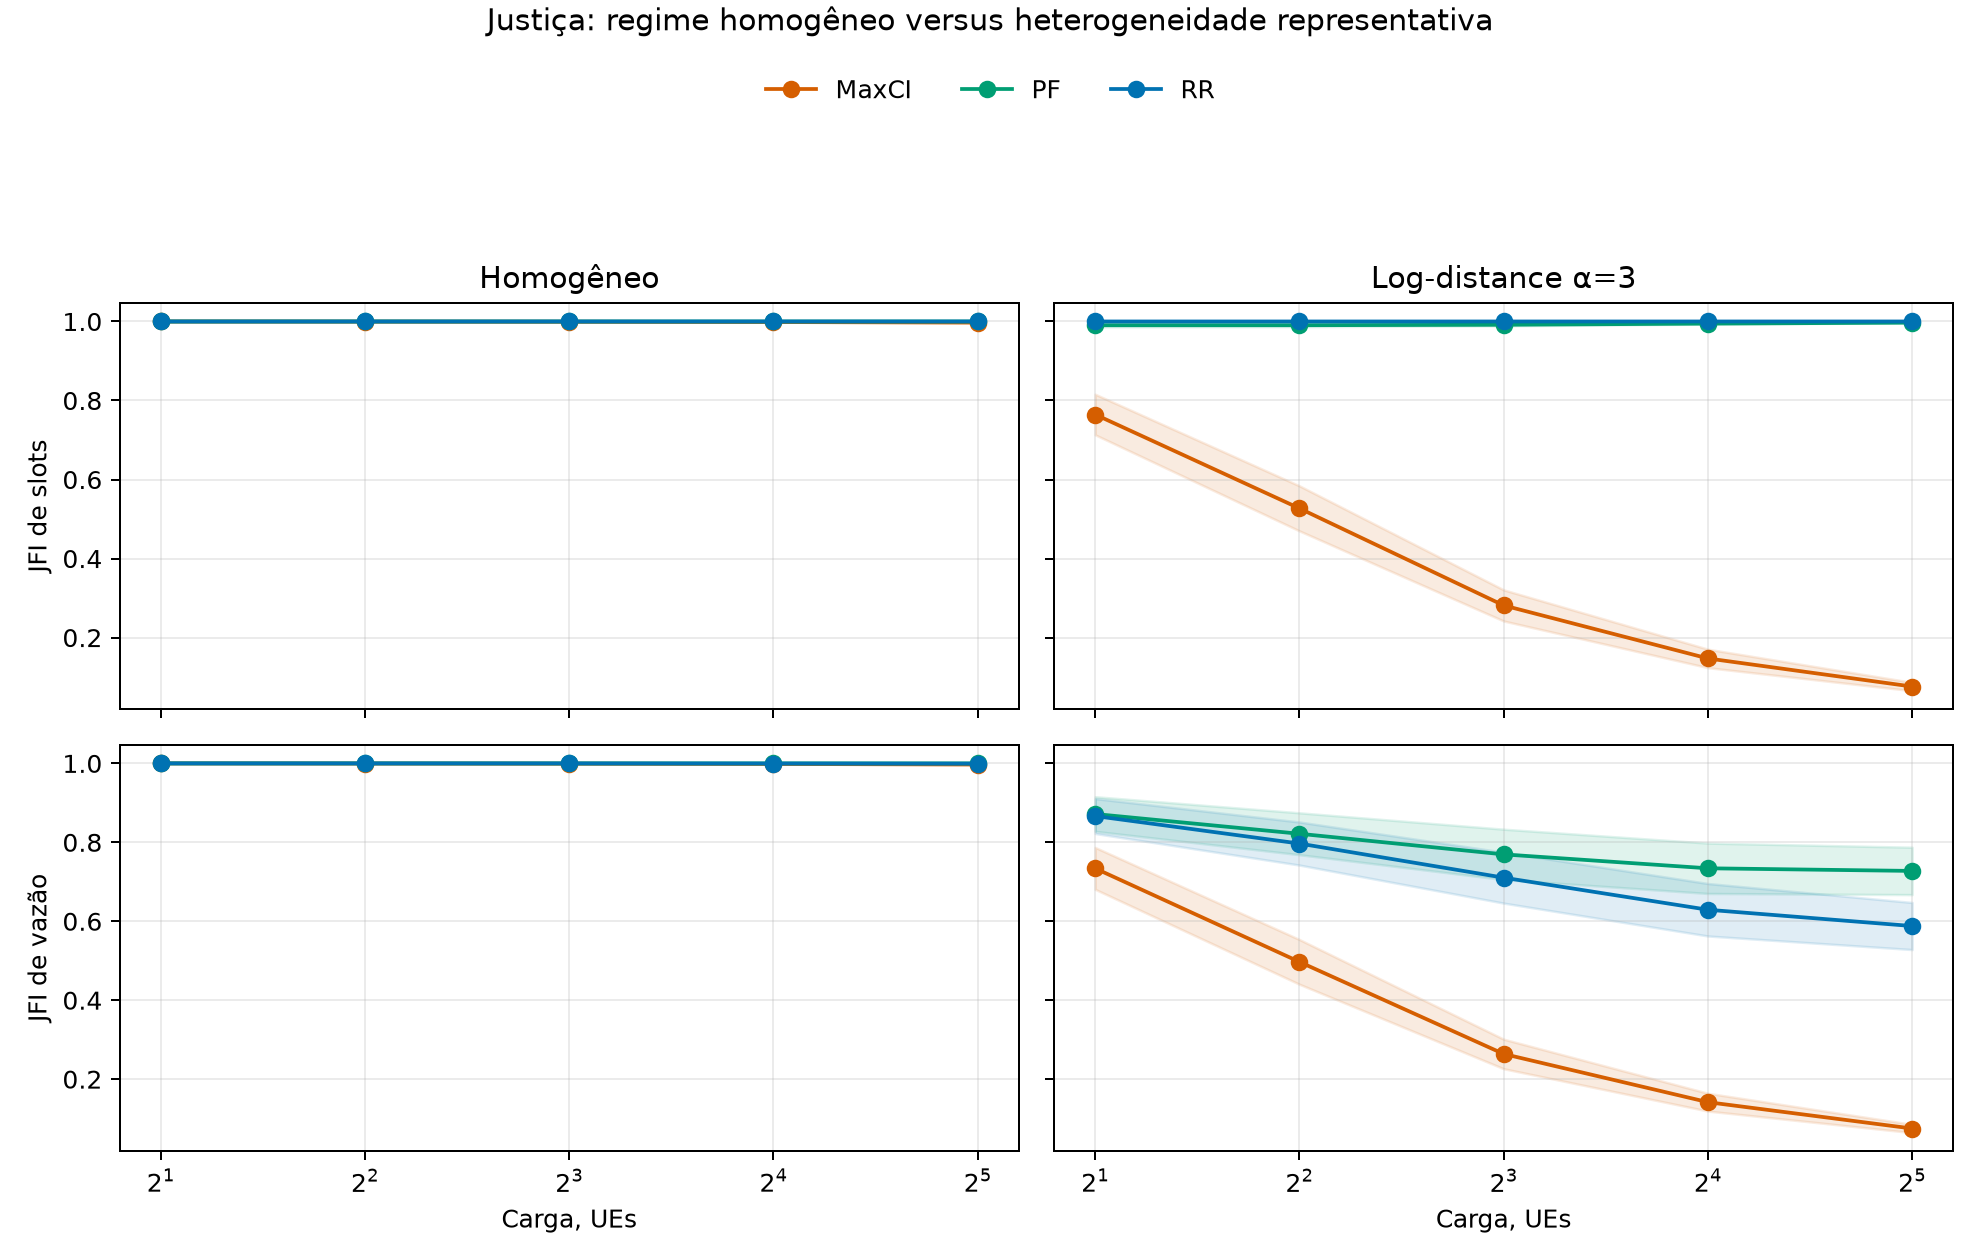
\includegraphics[width=1\linewidth]{figures/jfi_cenarios.png}

\end{figure}
\end{frame}


%------------------------------------------------
\begin{frame}{Eficiência x Justiça}

\textbf{Cenário mais extremo} (N=32, $\alpha=3$)
\begin{table}[htbp]
\centering
\small
\label{tab:extreme_scenario}
\begin{tabular}{lccccc}
\hline
Política & JFI slots & JFI vazão & Vazão célula & P5 vazão & UEs excluídos \\
\hline
RR       & 1,000     & 0,588     & 29,26        & 0,371    & 0,0           \\
PF       & 0,997     & 0,728     & 53,31        & 0,875    & 0,0           \\
MaxCI    & \textcolor{red}{0,076} & \textcolor{red}{0,075} & \textcolor{blue}{109,41} & \textcolor{red}{0,000} & \textcolor{red}{19,7} \\
\hline
\end{tabular}
\end{table}

\begin{itemize}

    \item MaxCI entrega a maior vazão agregada (109,41 Mbit/s), o dobro de PF e quase 4x RR;
    \item Mas em média 19,7 dos 32 usuários nunca são atendidos (exclusão total);
    \item Percentil 5 de vazão é zero, a cauda inferior colapsa.

\end{itemize}

\end{frame}

%%%%%%%%%%%%%%
% ADICIONAR GRÁFICOS AOS RESULTADOS...
%%%%%%%%%%%%%%

%------------------------------------------------

\begin{frame}

\begin{figure}[htp!]
\centering
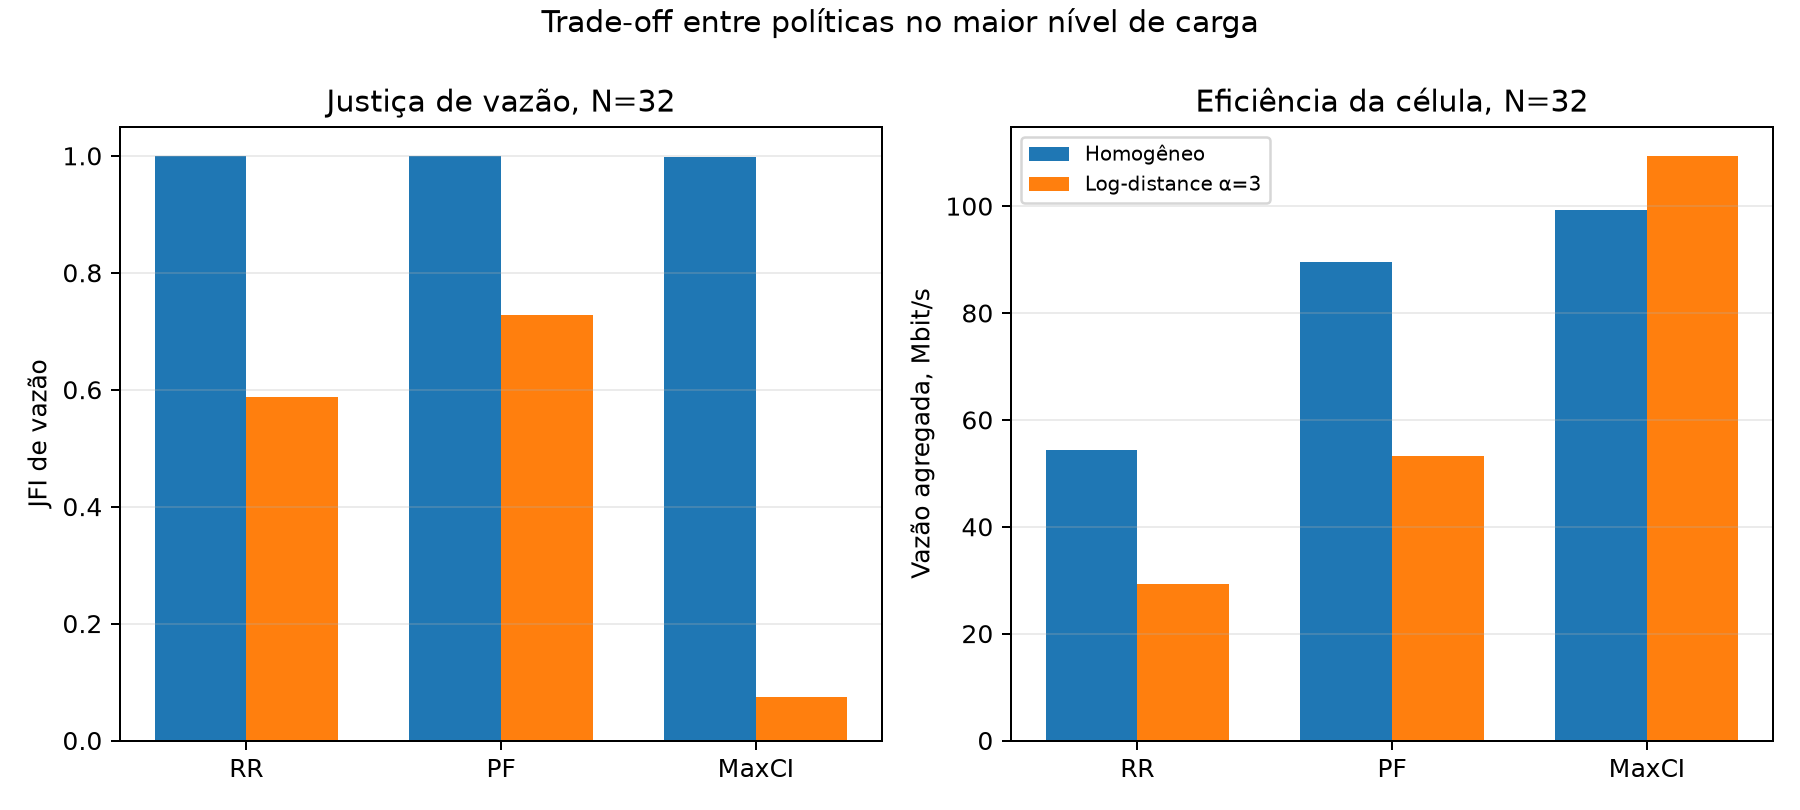
\includegraphics[width=1\linewidth]{figures/tradeoff_n32.png}
\end{figure}
\end{frame}


%------------------------------------------------
\section{Limitações}
\begin{frame}{Limitações} 
    \begin{itemize} 
        \item Cenário simplificado: \textbf{célula única e SISO}.
 
        \item Tráfego \textbf{full-buffer} e taxa baseada em modelo de Shannon. 
        
        \item Modelo de heterogeneidade baseado em \textbf{log-distance}, sem representar um cenário completo do 3GPP. 
        
        \item Não foram considerados: 
        \begin{itemize} 
            \item interferência intercelular; 
            \item shadowing; 
            \item mobilidade; 
            \item HARQ; 
            \item orçamento de enlace completo. 
        
        \end{itemize} 
    
    \item Resultados condicionados ao \textbf{cenário controlado analisado}. 
    \end{itemize} 
    
\end{frame}

%------------------------------------------------
\section{Conclusão}
\begin{frame}{Conclusão} 
     \begin{itemize} 
         \item No cenário homogêneo, o aumento da carga não provocou colapso de justiça no \textbf{MaxCI}. 
         \item A \textbf{heterogeneidade do canal} alterou esse comportamento, aumentando a vazão do MaxCI, mas também a concentração do serviço. \item O \textbf{RR} garantiu distribuição regular dos recursos, porém não equalizou a vazão entre os UEs. 
         \item O \textbf{PF} apresentou o melhor equilíbrio entre \textbf{vazão e justiça} no cenário heterogêneo. 
    \end{itemize} 
    \vspace{0.3cm} 
    \begin{block}{Conclusão principal} A escolha do scheduler deve considerar não apenas a vazão, mas também a heterogeneidade do canal e a métrica de justiça adotada. 
    \end{block} 
\end{frame}

%------------------------------------------------
\section{Bibliografia}
%------------------------------------------------

\begin{frame}
\frametitle{Referências}
\small
\begin{thebibliography}{99}

\bibitem[3GPP, 2020]{3GPP2020}
3GPP (2020). 
Study on channel model for frequencies from 0.5 to 100 GHz. 
Technical Report (TR) 38.901, 
3rd Generation Partnership Project (3GPP). 
Modelo UMi NLOS eq 7.4-7: PL = 36.7 log10(d3D) + 22.7 + 26 log10(fc).

\bibitem[Hoydis et al., 2022]{Hoydis2022}
Hoydis, J., Cammerer, S., Ait Aoudia, F., Vem, A., Binder, N., Marcus, G., and Keller, A. (2022). 
Sionna: An open-source library for next-generation physical layer research. 
O experimento usa Sionna 2.0.1 para geração do canal Rayleigh.

\bibitem[Jain et al., 1984]{Jain1984}
Jain, R. K., Chiu, D.-M. W., and Hawe, W. R. (1984). 
A quantitative measure of fairness and discrimination for resource allocation in shared computer systems. 
Research Report TR-301, Digital Equipment Corporation, Hudson, MA. 
Electronic reprint: arXiv:cs/9809099 (1998).

\bibitem[Lan et al., 2010]{Lan2010}
Lan, T., Kao, D., Chiang, M., and Sabharwal, A. (2010). 
An axiomatic theory of fairness in network resource allocation. 
In \emph{Proceedings IEEE INFOCOM}, pages 1–9.

\end{thebibliography}
\end{frame}

\begin{frame}
\frametitle{Referências}
\small
\begin{thebibliography}{99}

\bibitem[Mamane et al., 2022]{Mamane2022}
Mamane, A., Fattah, M., Ghazi, M. E., Bekkali, M. E., Balboul, Y., and Mazer, S. (2022). 
Scheduling algorithms for 5G networks and beyond: Classification and survey. 
\emph{IEEE Access}, 10:51643–51661.

\bibitem[Shi et al., 2005]{Shi2005}
Shi, H., Sethu, H., and Kanhere, S. S. (2005). 
An evaluation of fair packet schedulers using a novel measure of instantaneous fairness. 
\emph{Computer Communications}, 28(17):1925–1937.

\bibitem[Tse and Viswanath, 2005]{Tse2005}
Tse, D. and Viswanath, P. (2005). 
\emph{Fundamentals of Wireless Communication}, 
chapter 6 (Multiuser Diversity and Opportunistic Scheduling). 
Cambridge University Press.

\end{thebibliography}
\end{frame}


%------------------------------------------------
\section{}
%------------------------------------------------


%\setbeamertemplate{headline}{}
\begin{frame}
%\sffamily
\begin{center}
\HUGE \textcolor[RGB]{0,0,0}{Obrigado!}
\end{center}
\end{frame}



\end{document}



